% Pipeline

Since reference images maintain fixed headings and accurate GPS locations, adjustments for Earth's curvature are unnecessary in this context.
xxx - speak in intro abt why must reduce search space.  the image could have been distorted or messed up etc. 
    
feature extractors are nb bc they r iinvariant to scale rotation and transformation. As opposed to simply correlating entire image. also less computationally expensive.
https://baotramduong.medium.com/feature-extraction-in-computer-vision-using-python-358d7c9863cb



\section*{Planar Transforms}

When GPS is lost, the system relies on planar transforms to infer the UAV's location and heading based on these reference images. This is the key component to allow navigation back to base. Two primary approaches to estimate planar transforms are direct methods and feature-based methods, each with different strengths and limitations. \cite{lindenberger2023lightglue}

Direct methods use the entire image to estimate planar transforms by comparing pixel intensities and minimizing the differences through optimization techniques like gradient descent. While this makes them robust for small viewpoint changes, these methods are computationally expensive and can be sensitive to noise from bad pixels. However, the key limitation is that they work under an assumption of smooth, incremental movements between frames. When the UAV turns back to base, the large changes in rotation, perspective and translation cause the method to become unreliable. \cite{lindenberger2023lightglue}

In contrast, feature-based methods extract and match keypoints from both reference and real-time images, often using RANSAC to estimate planar transforms and reject outliers. This approach is more suitable for large viewpoint changes and rotations, as it does not rely on processing every pixel but focuses on distinctive features. Feature-based methods are computationally efficient and robust to large transformations and many forms of distortion. This makes them ideal for scenarios like this, where the UAV's flight path involves substantial changes in orientation and positioning. Therefore, feature-based methods were chosen for this system to ensure reliable navigation back to the base under varying conditions. \cite{lindenberger2023lightglue}

Feature-based matching involves feature detection, description, and matching. These matches form a point cloud which is used to estimate the planar transform. In this context, planar transformations involves the estimation of rotation and translation only, as per scope. Rotation and Translational estimations are tested separately, as they often require different strategies for optimal performance.  

The methods for each of these are chosen based on the following criteria: accuracy, speed, and robustness to different datasets and conditions. Further, the methods must be free to use, namely excluding state-of-the-art detectors SIFT and SURF, which require licensing fees. Finally, the methods must have credibility in the field, as they are used in a safety-critical application.






%https://mikhail-kennerley.medium.com/a-comparison-of-sift-surf-and-orb-on-opencv-59119b9ec3d0


\section{Feature Detectors}

Feature extraction is pivotal in image-based UAV navigation, enabling the estimation of transformations such as rotation and translation between consecutive images. Feature extractors identify \textbf{keypoints}—distinct, repeatable points within an image—and generate \textbf{descriptors} that encode information about the local image region surrounding each keypoint. These keypoints and descriptors facilitate accurate matching across multiple frames, allowing the system to track movement while maintaining invariance to changes in scale, rotation, and illumination. This precision is essential for accurately inferring both rotational and translational shifts between images.

The selected feature extractors—\textbf{ORB}, \textbf{AKAZE}, and \textbf{SuperPoint with LightGlue}—represent a diverse spectrum of approaches, offering different levels of accuracy, computational efficiency, and machine learning integration. Alternative methods were excluded to maintain scope or due to licensing fees. 

\subsection{Types of Feature Extractors}

\subsubsection{ORB (Oriented FAST and Rotated BRIEF)}
\textbf{ORB} combines the \textbf{FAST} keypoint detector with the \textbf{BRIEF} descriptor, enhanced for rotation invariance. \textbf{FAST} rapidly identifies keypoints by analyzing pixel intensity differences in a circular region around each candidate point. Once detected, \textbf{BRIEF} encodes the local image patch into a binary string through intensity comparisons. ORB adds rotational invariance by aligning keypoints based on their dominant orientation before descriptor computation. This makes ORB both fast and robust to scale and in-plane rotation, although it may struggle with repetitive textures or complex lighting variations.

\subsubsection{AKAZE (Accelerated-KAZE)}
\textbf{AKAZE} constructs a nonlinear scale space using diffusion-based filtering, capturing finer image details more effectively than linear methods. It detects keypoints by assessing local contrast with a specialized adaptive filter, enabling the identification of subtle features that simpler detectors might miss. The \textbf{Modified Local Difference Binary (MLDB)} descriptor encodes the neighborhood of each keypoint into a binary vector based on pixel intensity differences. While AKAZE is both fast and compact, its performance can be sensitive to detection thresholds across different environments. To ensure consistency, dynamic thresholding is applied, adjusting based on the environment to maintain a stable number of keypoints across diverse datasets.

\subsubsection{SuperPoint with LightGlue}
\textbf{SuperPoint} is a deep learning-based keypoint detector and descriptor that leverages convolutional neural networks (CNNs) to identify and describe keypoints in a single forward pass. Pre-trained on extensive image datasets, SuperPoint excels at recognizing stable and distinctive keypoints under varied conditions. \cite{rpaultrat2023superpoint} However, its performance may degrade on datasets significantly different from its training data. Pairing SuperPoint with \textbf{LightGlue}, a machine-learning-based matcher, enhances matching accuracy through advanced graph-based techniques. \cite{cvg2023lightglue} Despite their high accuracy, SuperPoint and LightGlue are computationally intensive, necessitating GPU acceleration for real-time applications; They are tested primarily to see if they subtend significantly more accurate results. During the testing phase, LightGlue was evaluated alongside SuperPoint and not retested during the matcher evaluation. 



\subsection*{Application}

Feature detectors were applied at four distinct stages in the UAV image-processing pipeline. Each stage addressed a specific need in the transformation estimation process. Different stages required different levels of precision and accuracy. The goal of the detector phase was to identify the efficiency and accuracy of each detector, and apply them accordingly to the subsequent stages.

For this reason there were the following tests conducted
efficiency
accuracy and robustness + generalizability - for BOTH rotation and translation estimations isolated via pass through to error. 




In the first stage, rotation between images was estimated to align them for similarity comparisons. While accuracy was necessary, runtime efficiency took priority due to the volume of image comparisons involved. Small rotational errors were acceptable, as global matchers, as tested later, showed tolerance to rotational inaccuracies. Thus, precise testing was not necessary. ORB with 6000 keypoints was chosen for this stage due to its efficiency and reasonable accuracy.

In the second stage, the goal was to use matches between images to estimate global context image similarity, focusing on the number of similar matches across grid extractions. Precision was less important here, but efficiency was paramount. ORB with 1500 keypoints was employed for this purpose. This stage’s efficiency in global similarity comparison was validated in the global matching section.

The first two stages were not explicitly tested for detector choice, as their performance largely depended on efficiency, where ORB clearly outperformed others. The focus in testing was on the latter two stages, which required higher precision.

In the third stage, accurate rotational estimation was prioritized to ensure proper alignment for translation estimation and heading output. 

In the fourth stage, precise translation estimation was needed for GPS inference. High accuracy was essential, as this stage directly affected the accuracy of positional data.

Empirical tests showed that the detector and corresponding parameter set that yielded the best translational estimate is not necessarily the best for rotational estimation. Different detectors prioritize different feature types, e.g. edges, that may suit one transformation more than another. Further, different transformations may handle the balance between number and quality of keypoints differently. Ultimately, the detector type and detection threshold must be independently found for rotational and translational estimates. 

It is for this reason tests must be conducted to find the optimal detector and parameters therefor in terms of accuracy, robustness and runtime for both rotation and translation estimation.



\subsection*{Application}
Feature detectors are used in four stages. The first is to find the rotation between images to align them for subsequent image similarity comparison. The second, is in the case when a local retrofit is used to find image similarity on a global context. The third, to find the accurate rotation change. The fourth, the accurate translation change. 
The first stage requires that rotation is calculated between the image to which inference is being done, and every reference image in the search space. As seen in the global matcher sections, these global techniques are invariant to small errors in rotational estimation. Since we are comparing multiple images, and rotational accuracy is not crucial, there is some ability to prioritize efficiency over accuracy. For this reason ORB is chosen due to its efficiency. ORB is used with 6000 keypoints. 
In the second, the matches need not be accurate, as a rough idea of the amount of matches that correspond is essential and no susbsequent inference is needed. A very crude ORB matches is used with a target of 1500 keypoints.
The third and fourth stage require accurate estimation of rotation and translation. Upon empirical testing, it was found that the detector that subtended the optimal point cloud for one piece of the transformation, did not always subtended the optimal detector for the other. Specifically, the best detector for rotation was also that for translation and vice versa. This is shown in appendix table \ref{tab:rot_reestimation}. AKAZE was shown as above to be the best for pure translation estimation and therefore dynamic keypoint target AKAZE with 3000 keypoints was chosen since the single image comparison does not require as much runtime prioritization. Since ORB performs better for the rotation estimate in general as seen in the table below, it is used. 


proof that the best detector for rotation is not also the best for translation.
TABLE:
\begin{table}[H]
    \centering
    \caption{RMSE and Runtime Comparison}
    \label{tab:rot_reestimation}
    \begin{tabular}{|c|c|c|}
    \hline
    \textbf{Dataset} & \textbf{RMSE (m)} & \textbf{Runtime (s)} \\ \hline
    \multicolumn{3}{|c|}{\textbf{WITH REESTIMATION OF ROTATION}} \\ \hline
    DATSETROT       & 67.7480           & 132.97               \\ \hline
    DATSETCPT       & 7.0124            & 131.52               \\ \hline
    DATSETROCK      & 24.6322           & 104.86               \\ \hline
    DATSETSAND      & 35.1589           & 107.22               \\ \hline
    DATSETAMAZ      & 37.3642           & 93.88                \\ \hline
    \multicolumn{3}{|c|}{\textbf{WITHOUT REESTIMATION OF ROTATION}} \\ \hline
    DATSETROT       & 68.0951           & 120.57               \\ \hline
    DATSETCPT       & 8.6607            & 100.08               \\ \hline
    DATSETROCK      & 23.2621           & 102.23               \\ \hline
    DATSETSAND      & 31.9800           & 91.50                \\ \hline
    DATSETAMAZ      & 40.0016           & 84.02                \\ \hline
    \end{tabular}
    \end{table}
    


\section{Feature Matching}

Feature matching establishes correspondences between keypoints in different images. After identifying these correspondences, ambiguities are removed to retain only the most reliable matches, which are then used to estimate transformations such as translation and rotation. This filtering ensures that transformation estimations are based solely on mutual information between images.

Unlike global matching methods, which assess the entire image context, \textbf{local feature matching} focuses on individual keypoints. This approach enables noise-invariant geometric transformations without relying on the assumption that most information is shared between images. Consequently, locally matched features are preferred for precise inference, while global matching is preferred for efficient image similarity comparisons.

Each matcher generates a list of potential matches along with their similarity scores, quantified using a descriptor-space distance metric. These scores help in determining the quality of the matches and play a crucial role in the subsequent filtering and transformation estimation processes.

\subsection{Types of Feature Matchers}

Two primary feature matchers are employed: the \textbf{Brute-Force Matcher (BFMatcher)} and the \textbf{Fast Library for Approximate Nearest Neighbours (FLANN)}. Additionally, \textbf{LightGlue}, a machine-learning-based matcher, is utilised for its enhanced accuracy despite its higher computational demands.

The \textbf{Brute-Force Matcher} compares each feature in one image with every feature in the second image, ensuring the best possible match. While this guarantees accuracy, it is computationally expensive, especially with large numbers of keypoints. \textbf{FLANN}, on the other hand, accelerates the nearest neighbour search in high-dimensional descriptor spaces using KD-trees or clustering algorithms. This approximate matching approach offers significant speed improvements with minimal loss in accuracy, making it ideal for real-time applications with many datapoints. \textbf{LightGlue} leverages deep learning to improve matching accuracy further. Although highly effective, its structure necessitates using it in conjunction with other neural network-based feature extractors like SuperPoint to realize its full potential. This matcher is tested in conjunction with SuperPoint during the detector testing phase and is not retested during the matcher testing phase.

\subsection{Search Techniques}

The search technique determines which potential matches are retained for further processing. Various methods, including \textbf{Radius Search}, \textbf{Vanilla Matching}, and \textbf{K-Nearest Neighbours (KNN) Matching}, are explored to control the number and quality of matches.

\textbf{Radius Search} retains matches within a specified distance in descriptor space, effectively filtering out weaker matches. However, it does not guarantee a fixed number of matches per keypoint, leading to inconsistent results. Due to this limitation, radius search was excluded from further experiments.

\textbf{Vanilla Matching} returns the single best match for each keypoint. Empirical testing demonstrated that this approach provided poor accuracy because it fails to remove ambiguities effectively, resulting in unreliable matches. Consequently, vanilla matching was not pursued further.

\textbf{K-Nearest Neighbours (KNN) Matching} retains the top \( K \) matches for each keypoint, allowing the application of post-filtering techniques such as Lowe’s ratio test to eliminate ambiguous matches. Matches with only one neighbour were discarded to avoid compromising accuracy when Lowe’s ratio could not be applied. Empirical tests indicated that values of \( K \) above 2 introduced impractical computational overheads. Therefore, \( K=2 \) was selected for subsequent experiments, balancing match quality and computational efficiency.

\textbf{Cross-Check Filtering} accompanies the above search techniques by ensuring that matches are mutual; only those matches that are consistent in both directions are retained. This mutual verification reduces the likelihood of false positives by ensuring that each match is one-to-one, thereby increasing the reliability of the correspondences. This was not pursued due to exorbitant computational costs.


\section{Image Similarity Computation}

Selecting the most similar reference image is critical for accurately inferring the UAV's current location. This process involves comparing the current image captured by the UAV with all images stored in the database to identify the one with the highest similarity. While geographical proximity often correlates with image similarity, factors such as image distortion or significant UAV movement can disrupt this relationship, necessitating robust similarity measures.

\subsection{Search Space Reduction}

To achieve real-time performance, the search space is initially narrowed to a subset of images likely to be similar to the current image. This reduction is based on the UAV's last known location, filtering images within a dynamic search radius that adapts to the UAV's speed and frame rate. Instead of using a fixed radius, which may be unsuitable across varying conditions, the radius expands incrementally until a predefined number of potential matches—typically five—are identified. This approach balances computational efficiency with the need to minimize the inclusion of irrelevant images.

\subsection{Global Matching Techniques}

Once the search space is reduced, a more precise similarity computation is performed on the remaining candidates to ensure accurate localization. This step must be both efficient and effective in capturing the overall context of the images. Prior to comparison, images are aligned to account for any rotational discrepancies, ensuring that similarity metrics are not adversely affected by misalignment.

Several global matching techniques are employed to evaluate image similarity:

\subsubsection{Local Detectors and Matcher Conversion Techniques}

Local feature matching involves identifying keypoints in both images and determining correspondences based on descriptor similarity. However, this method alone does not guarantee an even distribution of matches across the image, potentially leading to biased similarity scores. To address this, grid matching is applied, dividing the image into grids and limiting the number of matches per grid. Although computationally intensive, this technique enhances robustness against distortions and rotations by ensuring a uniform distribution of matches. In practice, ORB detectors combined with FLANN matchers have proven to be both accurate and efficient for this purpose.

\subsubsection{Cross-Correlation}

Cross-correlation measures similarity by sliding one image over another and computing the sum of pixel-wise multiplications at each position. The peak value indicates the best alignment, reflecting the highest similarity. While straightforward, this method is sensitive to noise and illumination changes, which can affect the reliability of the similarity measure.

\subsubsection{Histograms}

Histogram comparison assesses similarity by analyzing the distribution of pixel intensities. Each image's histogram is divided into bins (typically 256 for 8-bit images), and the similarity is quantified using metrics such as Chi-Square or Bhattacharyya distance. This method focuses on global color and brightness distributions but ignores spatial information, making it less effective for images with similar color profiles but different structures.

\subsubsection{Structural Similarity Index (SSIM)}

SSIM evaluates similarity by decomposing images into luminance, contrast, and structure components. It computes local statistics within small windows and combines them into a single similarity score that reflects perceived image quality. SSIM effectively captures structural information like edges and textures, aligning well with human visual perception. This makes it a robust choice for measuring image similarity in varied conditions.





\section*{Planar Transformation Estimators}

This section outlines the primary planar transformations used to compute the UAV's change in motion, specifically focusing on changes in rotation and translation derived from reference images. While the main goal is to estimate both rotation and translation, rotational estimation is also used independently in other stages of the pipeline. This process helps infer the UAV's location and heading. The estimators were carefully chosen for their balance of computational efficiency and accuracy, ensuring robust performance in the navigation system.

The transforms are applied onto matched points. To further improve the final GPS and heading inference, an important enhancement was introduced by splitting the final transformation estimation into two stages. First, the overall alignment between images is computed, followed by rotational alignment of one image to the other. This step implicitly removes non-common information, significantly reducing false positive matches. After this, matching and filtration are reapplied to the refined images, resulting in a substantial improvement in accuracy.

\subsection{Affine Transformation}

Affine transformation captures translation, rotation, scaling, and shear, providing six degrees of freedom. It is computed by estimating the affine transformation matrix between two sets of points using OpenCV. RANSAC is used to handle outliers by selecting random subsets of keypoints and fitting them to the affine model. RANSAC is also applied to the other OpenCV transformations, including Partial Affine and homography transformations. \cite{opencv_warp_affine}


\subsection{Rigid Transformation Estimation (SVD)}

Rigid transformation preserves the shape and size of objects by estimating only rotation and translation, excluding scaling and shear. Using Singular Value Decomposition (SVD), it minimizes the least-squares error between two point sets. This involves computing the weighted centroid of both point sets, centres the points by subtracting their centroids. Thereafter, the covariance matrix is computed, followed by Singular Value Decomposition (SVD) and subsequently used determine the rotation matrix. Finally, the translation vector is computed. This method is computationally efficient and well-suited for this application, where only rotation and translation are required. This method is computationally efficient and well-suited for this application, where only rotation and translation are required. \cite{sorkine2017least_squares}


\subsection{Partial Affine Transformation}

Partial affine transformation reduces the full affine model by focusing solely on translation and rotation, offering three degrees of freedom. It strikes a balance between the complexity of affine transformations and the limitations of rigid transformations. Using OpenCV in conjunction with RANSAC, it is ideal for this application, where only rotation and translation are important. \cite{opencv_warp_affine}

\subsection{Homography Transformation}

Homography transformation captures translation, rotation, scaling, shear, and perspective distortion, offering eight degrees of freedom. It is estimated using OpenCV, with RANSAC applied for outlier rejection. While homography provides greater flexibility, its additional degrees of freedom introduce unnecessary errors and computational overhead for this application, where only rotation and translation are required. \cite{opencv_homography}




\subsection*{Rotational Normalization Strategies}

Rotational normalization is essential for aligning images and translating estimations accurately in image-based UAV navigation systems. Two primary strategies were considered for normalizing rotations during the flight back to the base. The first involves applying rotational normalization during image capture, which aligns both images to a global North-East (NE) reference space before keypoint detection. The second method avoids normalization at the point of capture, aligning the images relative to one another and applying normalization only after translation estimation.

The key difference between these two methods lies in their respective losses caused by image rotation, due to the fixed canvas size during normalization. When an image is rotated, parts of the image are lost or moved off-canvas, particularly as the rotation approaches 90 degrees (a loss of 43.75\% for an aspect ratio of 16:9). This introduces information loss, which negatively impacts the accuracy of keypoint detection and translation estimation.

The loss function for the first approach, where images are normalized independently, is proportional to:

\begin{equation}
\text{Loss}_{\text{pre}} \propto |\sin(|\Delta_1|) + \sin(|\Delta_2|)|
\end{equation}

where \( \Delta_1 \) and \( \Delta_2 \) are the respective rotation angles of the two images relative to the global coordinate system. This results in compounded losses, as both images are treated independently. The maximum loss occurs when both images are rotated by ±90 degrees, at which point the sum of sine values peaks, leading to maximum information loss.

In the second approach, where images are aligned relative to each other before normalization is applied, the loss function is:

\begin{equation}
\text{Loss}_{\text{post}} \propto |\sin(|\Delta_2 - \Delta_1|)|
\end{equation}


Here, the loss depends on the relative difference in rotation between the two images, reducing the potential for compounded information loss. In the given application, during the return flight to base, the UAV will generally undergo a near 180-degree rotation relative to the outbound path with an expected tolerance of ±20 degrees. Given this constraint, the loss functions of both approaches are as follows for various rotation scenarios:

\begin{figure}[H]
    \centering
    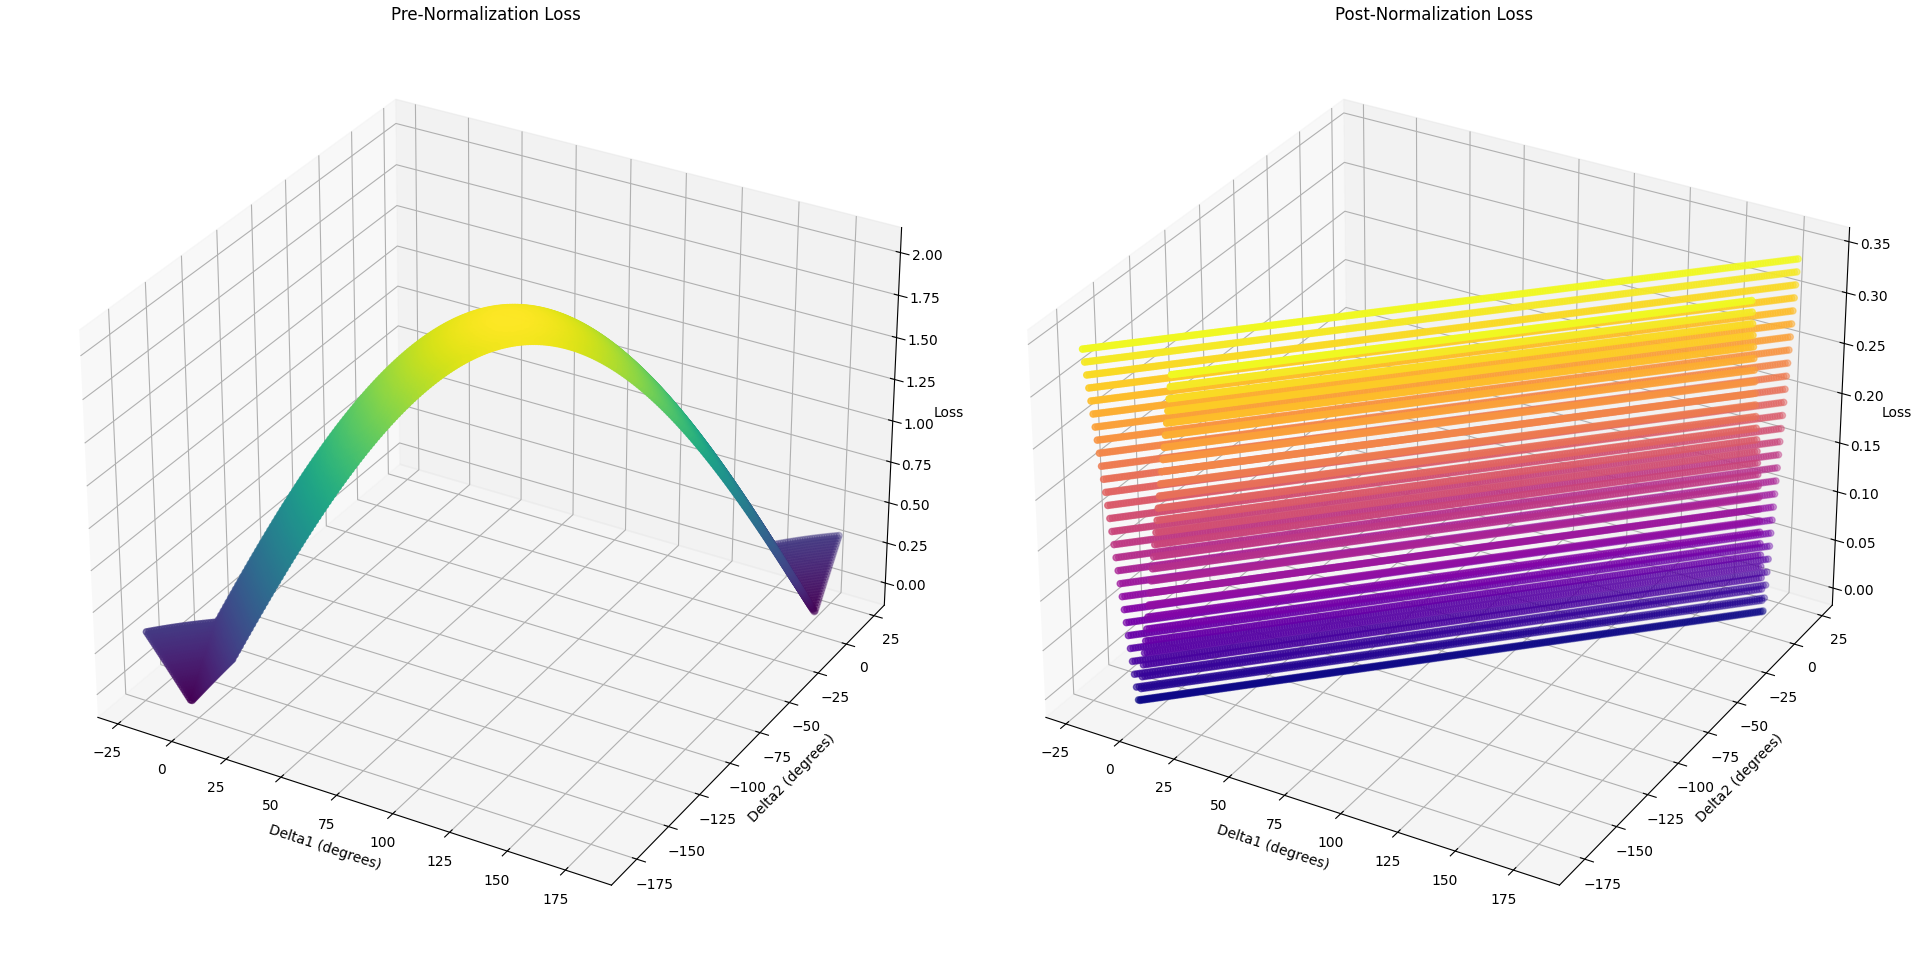
\includegraphics[width=\textwidth]{Chapter 4/Figs4/lossprevspost.png}
    \caption{Loss comparison between pre-normalization and post-normalization methods.}
    \label{fig:lossprevpost}
\end{figure}


As seen in Figure~\ref{fig:lossprevpost}, the pre-normalization method results in losses exceeding 2.0 due to the compounding effect of treating both images independently. In contrast, the post-normalization method, which works with relative rotation, consistently yields lower losses, with a maximum loss of approximately 0.35 under these typical UAV conditions. Therefore, post-normalization is expected to provide more accurate translation estimations due to better retention of keypoint information.




\subsubsection*{Empirical Validation}

In empirical tests, these results were confirmed, with post-normalization consistently providing higher accuracy due to better retention of keypoint information. The effects were most significant in the DESERT dataset, where the sparsity of keypoints made the dataset particularly sensitive to information loss during rotation. 

\subsubsection*{Method Conclusion}

Given the UAV's typical flight pattern and the need to minimize information loss, post-normalization is applied. In this approach, images are first aligned, followed by translation estimation. Finally, the translation vector is normalized to the global NE coordinate space for consistent navigation.









\section*{Optimization Techniques}

Optimizing parameter sets is crucial for enhancing the performance and robustness of the UAV navigation system. Given the significant variability in optimal parameters across different pipeline stages and datasets, an optimal, but not perfect, parameter configuration was determined for the entire pipeline. The objective was not to achieve the absolute best performance for each individual parameter set, as this would limit the system's generalizability and take extremely long. Further, if the method or pipeline does not perform well with a non-optimal parameter set, it is likely not robust enough to be used.

To maintain fairness and avoid parameter bias, methods were given parameters that ensure their own optimal operation.

\subsection*{RANSAC for Planar Transformation}
RANSAC (Random Sample Consensus) for planar transformation is a robust estimation technique that iteratively selects random subsets of point correspondences to fit a model and identify inliers. By randomly choosing a few point pairs, RANSAC estimates the affine transformation that fits these points and checks how well the remaining points align with the model. The method calculates the number of inliers—points that fit the transformation within a set threshold—and repeats the process for a predefined number of iterations or until it achieves a sufficient inlier ratio. This approach is highly effective in datasets with significant outliers, as it focuses on finding a model that works for the largest subset of inliers. However, due to its iterative nature and need to sample repeatedly, RANSAC can result in increased runtime, particularly in larger datasets or when dealing with numerous outliers.


\subsection{LMEDS (Local Maxima Extrema Density Selection) for Planar Transformation}
LMEDS (Local Maxima Extrema Density Selection) is a method designed to select keypoints based on areas of high feature density, identifying local maxima as keypoints for further matching. The technique focuses on regions where feature density peaks, selecting these local maxima to ensure the most significant and distinctive points are used in the matching process. By concentrating on areas of high feature concentration, LMEDS adapts to the feature distribution within the image, ensuring keypoints represent important regions while filtering out less significant points. This approach improves both accuracy and performance by reducing redundant keypoints and improving the quality of matches, particularly in areas with high feature variability. LMEDS is effective in outlier rejection, leading to more reliable transformations.


\subsection*{Lowe's Ratio Test}

Lowe's ratio test is utilized to filter keypoint matches based on the ratio of the distance of the best match to the second-best match. A match is retained if this ratio falls below a predefined threshold, indicating that the best match is significantly better than the alternatives. This test is essential for eliminating ambiguous or false matches, ensuring that only the most reliable correspondences are used in subsequent processing stages.

However, Lowe's ratio test is sensitive to the number and quality of detected keypoints. An excessively stringent ratio may discard valid matches, especially in scenarios with a high density of keypoints, while a lenient ratio might allow too many false positives. To address this, a dynamic thresholding approach was implemented. The threshold starts at a conservative value and is gradually relaxed until a sufficient number of matches is achieved. This strategy strikes a balance between minimizing false positives and ensuring enough reliable matches are available for stable transformation estimation. While there is a risk of introducing some false positives, this approach is necessary to maintain robustness across diverse datasets.

\subsection*{Parallel Flow Filtering}

Parallel Flow Filtering enhances match consistency by ensuring that feature matches align with the average motion flow resulting from the UAV's rotation and translation. In typical UAV movements, the flow of features is linear and parallel to the direction of motion, assuming no scale as per scope. This technique calculates an average motion vector by combining mean and median motion vectors and filters out matches that deviate beyond a specified angular threshold from this average flow. By removing inconsistent matches, Parallel Flow Filtering ensures that only matches conforming to the expected motion pattern contribute to the transformation estimation, thereby improving overall accuracy and reliability.

\subsection*{n-Match Thresholding} 
This method involves setting a threshold based on allowing a specific number of matches with the smallest descriptor distances. 

\subsection*{Absolute Thresholding of Matches} 
Absolute thresholding filters matches based on a fixed distance in descriptor space, retaining only those matches that meet a minimum closeness criterion. 


